\chapter{Convex conjugates}
\label{chap:convex_conjugates}

This chapter introduces a concept that is deeply connected to subgradients and
proximal mappings (as covered in the last two chapters), and to duality theory
(as will be covered next). In fact, just as with subgradients, proximal maps,
and duality, the topic of the current chapter is at the same time quite simple
and quite powerful.      

\section{Definition and properties}

Given a function $f : \R^d \to [-\infty, \infty]$, its \emph{convex conjugate}
$f^*$ (also simply called its conjugate) is another function on $\R^d$ defined
as        
\index{conjugate}
\begin{equation}
\label{eq:conjugate}
f^*(u) = \sup_x \, \Big\{ u^\T x - f(x) \Big\}.
\end{equation}
The mapping from $f \mapsto f^*$ is also called the \emph{Legendre-Fenchel
  transform}. At the outset, we remark that $f^*$ is always convex, by the
partial supremum rule in Property \parref{par:function_supremum} (the map
$u \mapsto u^\T x - f(x)$ is affine and thus convex for each $x$). 
Moreover, the function $f^*$ is always closed, since its epigraph can be
expressed as an intersection of closed halfspaces, which is a closed set
(Exercise \ref{ex:conjugate_closed}). To be clear, these properties---the
closedness and convexity of $f^*$---hold regardless of whether $f$ itself is
closed or convex.      

A useful interpretation of $f^*$ is as follows: at each point $u$, the value
$f^*(u)$ is the maximum gap between a linear function with ``slope'' $u$ and
$f$. Figure \ref{fig:conjugate} gives an illustration. This interpretation
suggests that there may be some interesting geometry at play that underlies the
convex conjugate, which we revisit shortly when we discuss double conjugation.      

\begin{figure}[tb]
\centering
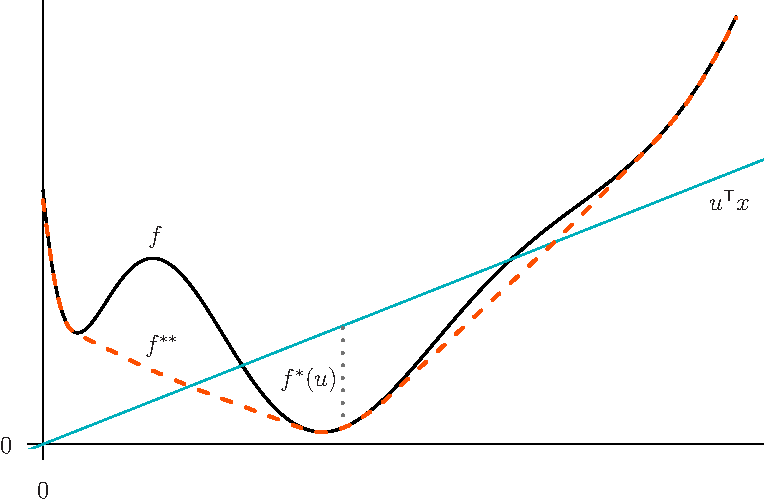
\includegraphics[width=0.7\textwidth]{fig/conjugate.pdf}
\caption{The conjugate $f^*$ evaluated at $u$ is the maximum gap between a
  linear function with slope $u$ and $f$, illustrated by the dotted line. The
  double conjugate $f^{**}$ is the pointwise supremum of all affine minorants to
  $f$ (equivalently, the greatest closed convex minorant to $f$), illustrated by
  the dashed line.}     
\label{fig:conjugate}
\end{figure}

Next we describe several important properties of convex conjugates. We generally
assume that $f \not= \infty$ ($\dom(f) \not= \emptyset$) henceforth to avoid 
trivialities when studying convex conjugates.        

\paragraph{Fenchel's inequality.}

For any $u$, observe that by the definition of the convex conjugate
\eqref{eq:conjugate} it holds that $f^*(u) \geq u^\T x - f(x)$, for any
$x$. Rearranging yields what is called \emph{Fenchel's inequality}, 
\index{Fenchel's inequality}
\begin{equation}
\label{eq:fenchel_inequality}
f(x) + f^*(u) \geq x^\T u, \quad \text{for all $x,u$}.
\end{equation}
Equality holds in \eqref{eq:fenchel_inequality} if and only if $x$ achieves the
supremum in \eqref{eq:conjugate}. As we show next, this can be further
characterized using subgradients of $f$.   

\paragraph{Subgradient equivalences.}

The supremum in \eqref{eq:conjugate} is attained at $x$ if and only if $x$
solves  
\[
\minimize_x \quad f(x) - u^\T x,
\]
which for convex $f$ is equivalent to $0 \in \partial f(x) - u$, that is, $u \in 
\partial f(x)$, using subgradient optimality. (Note that we use convexity 
of $f$ to split the subdifferential of a sum into a sum of subdifferentials, by 
Property \parref{par:subgradient_sum}.)  Meanwhile, by the rule for subgradients
of a partial supremum (Property \parref{par:subgradient_supremum}) we know that
$\partial f^*(u)$ contains all points of the form 
\[
\nabla_u \big( u^\T x - f(x) \big) = x,
\]
such that $x$ that achieves the supremum in \eqref{eq:conjugate}. In fact, if
$f$ is \emph{closed} and convex, then using the fact that $f^{**} = f$, to be 
established below, we can conclude that this describes \emph{all} of the
elements of $\partial f^*(u)$ (Exercise \ref{ex:conjugate_subgradients}). The 
next result records these equivalences. 

\index{conjugate!subgradients}
\begin{Theorem}
\label{thm:conjugate_subgradients}
For closed and convex $f$ with nonempty domain, the following statements are all 
equivalent:
\begin{enumerate}[label=(\roman*)]
\item $x$ achieves the supremum in \eqref{eq:conjugate};
\item $f(x) + f^*(u) = x^\T u$;
\item $u \in \partial f(x)$;
\item $x \in \partial f^*(u)$.
\end{enumerate}
\end{Theorem}
\vspace{-3pt}

\paragraph{Double conjugation.}

The conjugate of $f^*$ is known as the \emph{double conjugate} of $f$ and
denoted $f^{**}$. Simply applying the definition \eqref{eq:conjugate} with $f^*$
in place of $f$, we get 
\index{conjugate!double}
\begin{equation}
\label{eq:double_conjugate}
f^{**}(x) = \sup_u \, \Big\{ x^\T u - f^*(u) \Big\},
\end{equation}
and by the same rationale given previously, we note that $f^{**}$ is always
closed and convex. Applying Fenchel's inequality \eqref{eq:fenchel_inequality},
that is, $f^*(u) \geq x^\T u - f(x)$, to the term inside the supremum gives    
\[
f^{**} \leq f,
\]
or, in other words, the double conjugate $f^{**}$ minorizes the original
function $f$. In fact, the double conjugate function $f^{**}$ is not just any
(convex) minorant of $f$, it is the pointwise supremum of all affine minorants
of $f$ (Exercise \ref{ex:double_conjugate_affine_minorant}):       
\begin{equation}
\label{eq:double_conjugate_affine_minorant} 
f^{**}(x) = \sup \, \{ g(x) : \text{$g$ is affine, and $g \leq f$} \}, \quad
\text{for all $x \in \dom(f)$}. 
\end{equation}
See Figure \ref{fig:conjugate} again for an illustration. Finally, a special
reduction occurs for closed and convex $f$: in this case, we get that the double 
conjugate reduces to the original function, 
\begin{equation}
\label{eq:double_conjugate_identity}
f^{**} = f.
\end{equation}
Exercises
\ref{ex:affine_minorant_revisited}--\ref{ex:double_conjugate_identity} walk
through the proof of this and related facts.

\medskip

\begin{Example}
Below are examples of convex conjugates for some functions of interest. The
calculations for most are straightforward; for others we defer the details to
exercises.   

\begin{enumerate}[label=\alph*., ref=\alph*]
\item \parlab{xa:quadratic_conjugate}
  For $f(x) = \frac{1}{2} x^\T Q x$, where $Q \succ 0$, its conjugate is $f^*(u)
  = \frac{1}{2} u^\T Q^{-1} u$.  

\item For $f(x) = \sum_{i=1}^d \log(1+e^{x_i})$, its conjugate is 
  \[
  f^*(u) = \sum_{i=1}^d \big( u_i \log(u_i) + (1-u_i) \log(1-u_i) \big), 
  \] 
  with $\dom(f^*) = [0,1]^d$ (and where we interpret $0 \log(0) = 0$). 

\item For $f(x) = \sum_{i=1}^d x_i \log(x_i)$, its conjugate is $f^*(u) =
  \sum_{i=1}^d \exp(u_i - 1)$. 
\index{negative entropy function!conjugate}

\item \parlab{xa:characteristic_function_conjugate}   
  For $f = I_C$, the characteristic function of an arbitrary set $C$, its
  conjugate is \vphantom{$\sum_{i=1}^d$} 
  \index{characteristic function!conjugate}
  \[
  f^* = h_C,
  \]
  where recall \smash{$h_C(u) = \sup_{x \in C} \, u^\T x$} denotes the support
  function corresponding to $C$.  

\item \parlab{xa:support_function_conjugate} 
  For $f = h_C$, the support function corresponding to a closed, convex, and
  nonempty set $C$, its conjugate is (Exercise
  \ref{ex:support_function_conjugate}):    
  \index{support function!conjugate} 
  \[
  f^* = I_C,
  \]
  the characteristic function of $C$. 

\item \parlab{xa:norm_conjugate}  
  For $f(x) = \|x\|$, where $\|\cdot\|$ is an arbitrary norm, its conjugate is
  (Exercise \ref{ex:norm_conjugate}):  
  \index{norm!conjugate}
  \index{dual norm}
  \[
  f^* = I_{\{u \,:\, \|u\|_* \leq 1\}},
  \]
  the characteristic function of the unit ball in the dual norm
  $\|\cdot\|_*$.
\end{enumerate}
\end{Example}

\section{Conjugate calculus}

We describe rules that will be helpful in calculating convex conjugates.  

\paragraph{Scaling.}
\parlab{par:conjugate_scaling}

It helps to first introduce some notation: for a function $f$ and $a>0$, we 
write $af$ to denote the function defined by $(af)(x) = af(x)$, whereas we write
$fa$ for the function defined by $(fa)(x) = af(x/a)$. We refer to the operation
$f \mapsto af$ as \emph{left scaling}, and the operation $f \mapsto fa$ as
\emph{right scaling}.

Now we are ready to describe the relationship between scaling and conjugacy: for
any function $f$ and $a>0$, it holds that $(fa)^* = af^*$. Moreover, for closed 
and convex $f$, we have $(af)^* = f^*a$. In short, for closed and convex
functions, left and right scaling are dual operations under conjugacy. 

\paragraph{Translation.}

The simplest translation rule is as follows: for any function $f$ and $a \in
\R$, writing $f+a$ for the function defined by $(f+a)(x) = f(x)+a$, it holds
that $(f+a)^* = f^*-a$. That is, addition and subtraction by a real constant are
dual to each other.

Another translation rule: if $F(x) = f(x-a)$, for any $f$ and $a \in \R^d$, then
$F^*(u) = f^*(u) + a^\T u$, and if $F(x) = f(x) + a^\T x$, then $F^*(u) =
f^*(u-a)$. That is, translation of the domain by a vector $a$ and addition by a
linear function with ``slope'' $a$ are dual to each other. 

\paragraph{Linear composition.}

Similar to scaling, we first introduce some notation. For $A \in \R^{d \times
  k}$, and a function $f$ on $\R^d$, we write $fA$ to denote the function (on
$\R^k$) defined by $(fA)(x) = f(Ax)$. Also, for a function $f$ on $\R^k$, we
write $Af$ to denote the function (on $\R^d$) defined by 
\[
(Af)(y) = \inf_{Ax=y} \, f(x).
\]
We refer to the operation $f \mapsto Af$ as \emph{left composition}, and $f
\mapsto fA$ as \emph{right composition}.

Now we can describe the relationship between composition and conjugacy: for any
function $f$ on $\R^k$ and $A \in \R^{d \times k}$, it holds that $(Af)^* =
f^*A^\T$. Moreover, for a closed and convex function $f$ on $\R^d$, we have 
$(fA)^* = A^\T f^*$. In other words, for closed and convex functions, left and
right composition are dual to each other.     
\index{composition!conjugate}

\paragraph{Separable sum.}

If $F(x) = f_1(x_1) + f_2(x_2)$ for a block variable $x = (x_1, x_2)$, then
$F^*(u) = f_1^*(u_1) + f_2^*(u_2)$ for $u = (u_1,u_2)$. 

\paragraph{General sum.}
\parlab{par:conjugate_general_sum}

In order to explain what happens for a general sum of functions, which is one of
the most notable calculus rule for convex conjugates, we recall the notion of an
\emph{infimal convolution} of functions $f,g$ (first introduced in Exercise
\ref{ex:moreau_proximal_identification}):  
\index{infimal convolution!conjugate}
\begin{equation}
\label{eq:infimal_convolution}
(f \infconv g)(x) = \inf_z \, \Big\{ f(z) + g(x-z) \Big\}.
\end{equation}
For any $f,g$, a straightforward calculation shows that $(f \infconv g)^* = f^*
+ g^*$. Meanwhile, for closed and convex $f,g$ whose effective domains have
relative interiors have a point in common, it holds that $(f + g)^* = f^*
\infconv g^*$. That is, for such closed and convex functions, infimal
convolution and addition are dual operations to each other. This provides an
interesting perspective on the Moreau envelope (a special case of an infimal
convolution), which we return to in Chapter \ref{sec:moreau_revisited}.    

\section{Conjugates and smoothness*}
\label{sec:conjugate_smoothness}

The smoothness of a function $f$ and convexity properties of its convex
conjugate $f^*$ turn out to be strongly related. To explore these connections,
we must first define some concepts. A function $f$ on $\R^d$ is said to be
\emph{essentially smooth} if the following three properties hold, for $C =
\interior(\dom(f))$:    
\begin{enumerate}[label=(\roman*)]
\item $C \not= \emptyset$;
\item $f$ is differentiable on $C$;
\item $\lim_{k \to \infty} \|\nabla f(x_k)\|_2 \to \infty$ whenever $\lim_{k \to
    \infty} x_k \to x \in \boundary(C)$, and \smash{$\{x_k\}_{k=1}^\infty
    \subseteq C$}. 
\end{enumerate}
An important special case is a function that is finite and differentiable on all
of $\R^d$. It turns out for a closed convex function $f$ that condition (iii)
is equivalent to $\partial f(x) = \emptyset$ for $x \notin \interior(\dom(f))$.   

A function $f$ is said to be \emph{essentially strictly convex} if it is
strictly convex on all convex subsets $S$ of $ \{x : \partial f(x) \not=
\emptyset\}$. (Here we say $f$ is strictly convex on $S$ to mean that
\eqref{eq:strictly_convex_function} holds for $x,y \in S$.) An important special 
case is a function that is finite and strictly convex on all of $\R^d$. 
\index{strict convexity}

The next result shows that conjugacy provides the bridge between the last two
concepts.  

\begin{Theorem}
\label{thm:conjugate_essentials}
A closed convex function $f$ is essentially strictly convex if and only if $f^*$
is essentially smooth. 
\end{Theorem}

% Theorem 26.3 in Rockafellar (1970)

As $f^{**} = f$ for closed convex functions, we can also read off as a
conclusion from Theorem \ref{thm:conjugate_essentials} that $f$ is essentially
smooth if and only if $f^*$ is essentially strictly convex. The proof of Theorem 
\ref{thm:conjugate_essentials} is driven by the connection between subgradients
of $f$ and $f^*$ from Theorem \ref{thm:conjugate_subgradients}, and is outlined
in Exercise \ref{ex:conjugate_essentials}.

In fact, combined with the relationship between subgradients of $f$ and $f^*$,
Theorem \ref{thm:conjugate_essentials} leads to an interesting conclusion. To
make this conclusion more salient, we introduce one more definition: a function
said to be of \emph{Legendre type} if it is essentially smooth and essentially
strictly convex. Using this nomenclature, and the fact that $f^{**} = f$ for
closed convex functions, Theorem \ref{thm:conjugate_essentials} says that a
closed convex function $f$ is of Legendre type if and only if $f^*$ is. Theorem
\ref{thm:conjugate_subgradients} then says that for any such $f$ and $x \in
\interior(\dom(f))$, we have $u = \nabla f(x) \iff x = \nabla f^*(u)$. This is   
summarized next. 

\index{Legendre function}
\begin{Theorem}
\label{thm:conjugate_legendre}
A closed convex function $f$ is of Legendre type if and only if $f^*$
is. Moreover, for $f,f^*$ of Legendre type, the gradient map
\[
\nabla f : \interior(\dom(f)) \to \interior(\dom(f^*))
\]
is invertible, with inverse $(\nabla f)^{-1} = \nabla f^*$. 
\end{Theorem}

% Theorem 26.5 in Rockafellar (1970)

Lastly, beyond the above connections, there is a crisp quantitative connection
between convexity properties of $f$ and smoothness properties of $f^*$. 

\index{Lipschitz smoothness}
\index{strong convexity}
\begin{Theorem}
\label{thm:conjugate_smoothness}
Let $f$ be a closed convex function. Then $f$ is strongly convex with parameter
$m>0$ if and only if $\nabla f^*$ is Lipschitz with parameter $1/m>0$. 
\end{Theorem}

The proof of Theorem \ref{thm:conjugate_smoothness} is outlined in Exercise
\ref{ex:conjugate_smoothness}. Together, the results in Theorems 
\ref{thm:conjugate_legendre} and \ref{thm:conjugate_smoothness} explain the
apparent symmetry behind Theorems \ref{thm:lipschitz_smoothness} and
\ref{thm:strong_convexity}.    

\medskip

\begin{Example}
The duality between Lipschitz smoothness and strong convexity is illustrated
nicely by the quadratic function $f(x) = \frac{1}{2} x^\T Q x$, for $Q \succ
0$, where $f^*(u) = \frac{1}{2} u^\T Q^{-1}u$. Denote by
\smash{$\lambda_{\max}(A)$} and \smash{$\lambda_{\min}(A)$} the largest and
smallest eigenvalues, respectively, of a matrix $A \succeq 0$. Then the
following holds:
\begin{itemize}
\item the Lipschitz constant of $\nabla f$ is \smash{$\lambda_{\max}(Q)$},
  whereas the strong convexity constant of $f^*$ is
  \smash{$\lambda_{\min}(Q^{-1}) = 1/\lambda_{\max}(Q)$};
\item the strong convexity constant of $f$ is \smash{$\lambda_{\min}(Q)$},
  whereas the Lipschitz constant of $\nabla f^*$ is
  \smash{$\lambda_{\max}(Q^{-1}) = 1/\lambda_{\min}(Q)$}. 
\end{itemize}
\end{Example}

\section{Proximal connections*}

Conjugate functions bear a number of important connections to proximal maps,
which we describe in this section.

\subsection{Moreau decomposition}
\label{sec:moreau_decomposition}

A closed and convex function $f$ and its conjugate $f^*$ exhibit the following 
relationship between their proximal operators:    
\begin{align*}
z = \prox_f(x) &\iff x-z \in \partial f(z) \\
&\iff z \in \partial f^*(x-z) \\
&\iff x-z = \prox_{f^*}(x),
\end{align*}
where in the first and last we line used the subgradient characterization for the
proximal map \eqref{eq:proximal_subgradient_characterization}, and in the second
we used the relationship between subgradients of $f,f^*$ from Theorem
\ref{thm:conjugate_subgradients}. We can rewrite the above conclusion more
succinctly as    
\index{Moreau decomposition}
\begin{equation}
\label{eq:moreau_decomposition}
\prox_f(x) + \prox_{f^*}(x) = x, \quad \text{for all $x$}.
\end{equation}
called the \emph{Moreau decomposition} of the proximal maps of the conjugate
pair $f,f^*$. This generalizes the decomposition we saw earlier in
\eqref{eq:projection_decomposition} for a projection operator onto a linear 
subspace $L$ and its orthocomplement $L^\perp$.  

An extended version of the Moreau decomposition \eqref{eq:moreau_decomposition}
is obtained by applying this formula to $\lambda f$, then applying rules for
conjugates and proximal operators under scaling (Exercise
\ref{ex:moreau_decomposition_lambda}):    
\begin{equation}
\label{eq:moreau_decomposition_lambda}
\prox_{\lambda f}(x) + \lambda \prox_{\lambda^{-1} f*}(x/\lambda) = x, \quad  
\text{for all $x$}. 
\end{equation}
This is useful for deriving the proximal operator of a function given the
knowledge of the proximal operator of its conjugate. This demonstrated in
Exercise \ref{ex:linf_norm_proximal_mapping} for the $\ell_\infty$ norm and in 
Exercise \ref{ex:operator_norm_proximal_mapping} for the operator norm. 

\subsection{Moreau envelope, revisited}
\label{sec:moreau_revisited}

We saw from Property \parref{par:conjugate_general_sum} that infimal
convolutions are connected to conjugacy through addition: $(f \infconv g)^* =
f^* + g^*$ for any $f,g$. The Moreau envelope \eqref{eq:moreau_envelope_lambda}
is a special case of an infimal convolution \eqref{eq:infimal_convolution} with
\smash{$g = \frac{1}{2\lambda} \|\cdot\|_2^2$}, that is, \smash{$f_\lambda = f
  \infconv \frac{1}{2\lambda} \|\cdot\|_2^2$}. Thus we can apply the fact from
Property \parref{par:conjugate_general_sum} to give 
\[
f_\lambda^* = f^* + \frac{\lambda}{2} \|\cdot\|_2^2,
\]
where we used Example \parref{xa:quadratic_conjugate} for the conjugate of
\smash{$\frac{1}{2\lambda} \|\cdot\|_2^2$}. Meanwhile, if $f$ is closed, then
$f_\lambda$ is too (recall, it is differentiable, and hence continuous), so we
can take the conjugate of both sides above and apply
\eqref{eq:double_conjugate_identity} to conclude   
\index{Moreau envelope}
\begin{equation}
\label{eq:moreau_envelope_conjugate}
f_\lambda = \bigg( f^* + \frac{\lambda}{2} \|\cdot\|_2^2 \bigg)^*,
\end{equation}
which explains precisely how the Moreau envelope acts as a regularized version 
of $f$, via conjugacy. We can see clearly that a smaller value of $\lambda>0$
leads to a smaller amount of regularization. In fact, we might guess from 
\eqref{eq:moreau_envelope_conjugate} that as $\lambda \to 0$, we will have  
$f_\lambda\to f$ (recalling that $f$ is closed and convex, which means $f^{**} =
f$). This claim is indeed true, and Exercise \ref{ex:moreau_envelope_conjugate}
outlines its proof.    

\section{Existence of minima, revisited*}
\label{sec:conjugate_minima}
\index{optimization problem!existence of solutions}

Conjugacy provides a lens through which we can interpret the existence of
minima. To see this, we can revisit the previously established connections
between subgradients and conjugate functions: for closed convex $f$ with
nonempty domain, recall (Theorem \ref{thm:conjugate_subgradients}) that $x \in
\partial f(y) \iff y \in \partial f^*(x)$. In particular, taking $y = 0$ reveals
the following equivalence: $f$ has a minimizer at $x$ if and only if and only if
$x \in \partial f^*(0)$. In other words, the set of minimizers of $f$ is equal
to $\partial f^*(0)$, and hence, this set is nonempty provided $0 \in
\relint(\dom(f^*))$ (Theorem \ref{thm:subgradient_existence}).  

More can be said: the subdifferential $\partial f^*(0)$, and thus the set of
minimizers of $f$, is nonempty and bounded if and only if $0 \in
\interior(\dom(f))$ (Theorem \ref{thm:subgradient_boundedness}). Lastly, $f$ has
a unique minimizer if and only if $\partial f^*(0)$ is a singleton, which
happens if and only if $f^*$ is differentiable at zero (Theorem
\ref{thm:subgradient_uniqueness}). The next theorem collects these results, for
completeness.

\begin{Theorem}
For closed and convex $f$ with nonempty domain, the following holds.

\begin{enumerate}[label=(\roman*)]
\label{thm:conjugate_minima} 
\item The set $S^\star$ of minimizers of $f$ satisfies $S^\star = \partial
  f^*(0)$, and thus $f$ attains its infimum if and only $f^*$ is
  subdifferentiable at zero, which holds if $0 \in \relint(\dom(f^*))$.    

\item The set $S^\star$ is nonempty and bounded if and only if $0 \in
  \interior(\dom(f^*))$.   

\item The set $S^\star$ is a singleton if and only if $f^*$ is differentiable
  at zero. 
\end{enumerate}
\end{Theorem}
 
Exercise \ref{ex:conjugate_recession} explores the relation between the above
theorem and our previous analysis of the existence of minima (Chapter
\ref{sec:existence_minima}), involving directions of recession.   

\SkipTocEntry\section*{Chapter notes}

It is not uncommon for books on convex analysis and optimization to pass over
conjugacy, without placing too much emphasis on the topic. However,
\cite{hiriartUrruty2001fundamentals} (Chapter E), and especially
\cite{rockafellar1970convex} (Chapters 11, 12, 16, 26), are notable
exceptions. Rockafellar's own take on the central importance of conjugacy, as he 
explains in the preface to his book, was influenced by the (unpublished) lecture 
notes of Werner Fenchel \cite{fenchel1951convex}. In
\cite{rockafellar1970convex}, most of the derivations of conjugacy properties 
and relations are geometric in nature; Exercise
\ref{ex:affine_minorant_revisited} gives a glimpse of the power of this
perspective. The latter book also provides an extensive treatment of conjugate
calculus (Chapter 15), and functions of Legendre type (Chapter 26).

The Moreau decomposition is due to \cite{moreau1962fonctions,
  moreau1965proximite}, and the connection between the Moreau envelope and
regularization (the fact that $f_\lambda$ smoothly approximates $f$ as $\lambda
\to 0$) is due to \cite{attouch1977convergence}, which was later generalized by 
\cite{attouch1981convergence}.   

\clearpage

\begin{xcb}{Exercises}
\begin{enumerate}[label=\thechapter.\arabic*]
\settowidth{\leftmargini}{0.00.\hskip\labelsep}
\index{conjugate!epigraph}
\item \label{ex:conjugate_closed}
  Prove that the epigraph of $f^*$ in \eqref{eq:conjugate} can be expressed as  
  \[
  \epi(f^*) = \{ (u,s) : u^\T x \leq f(x) + s, \, \text{for all $x$} \},
  \]
  which as an intersection of closed halfspaces, and is hence closed. 

\index{conjugate!subgradients}
\item \label{ex:conjugate_subgradients}
  This exercise examines subgradients of the conjugate function.

\begin{enumerate}[label=\alph*.]
\item Show that $x \in \partial f^*(u)$ for any $x$ that achieves the supremum
  in \eqref{eq:conjugate}. Hint: recall the rule in Property
  \parref{par:subgradient_supremum}. 

\item When $f$ is closed and convex, show further that $x \in \partial f^*(u)$
  if and only if $x$ achieves the supremum in \eqref{eq:conjugate}. Hint: first
  show $x \in \partial f^*(u)$ if and only if $u$ achieves the supremum in
  \eqref{eq:double_conjugate}, by subgradient optimality. Then use the fact that
  $u$ achieves the supremum in \eqref{eq:double_conjugate} if and only if
  $f^{**}(x) + f^*(u) = x^\T u$. Lastly, reinterpret the last condition using
  the fact that $f^{**} = f$ for closed convex $f$. 
\end{enumerate}

\item \label{ex:double_conjugate_affine_minorant}
  We prove the fact in \eqref{eq:double_conjugate_affine_minorant}, for $x \in
  \dom(f)$, by proving separately that the left-hand side is at most and at
  least the right-hand side.     

\begin{enumerate}[label=\alph*.]
\item Prove that $f^{**}(x) \geq \sup \, \{ g(x) : \text{$g$ is affine, and $g
    \leq f$} \}$. Hint: if $g(x) = u^\T x + b$ satisfies $g \leq f$, then show
  that $f^*(u) \leq -b$, and thus $f^{**}(x) \geq u^\T x + b = g(x)$. 
  
\item Prove that $f^{**}(x) \leq \sup \, \{ g(x) : \text{$g$ is affine, and $g
    \leq f$} \}$. Hint: observe that $f^{**}(x)$ is the supremum of $g(x)$ over
  all affine minorants $g$ of the form $g(y) = u^\T y - f^*(u)$.  
\end{enumerate}

\item \label{ex:affine_minorant_revisited}
  This exercise proves a refined version of the fact from Exercise
  \ref{ex:affine_minorant}: for closed and convex $f$,  
  \begin{equation}
  \label{eq:affine_minorant_revisited}
  f(x) = \sup \, \{ g(x) : \text{$g$ is affine, and $g \leq f$} \}, \quad
  \text{for all $x \in \dom(f)$}.
  \end{equation}
 % Theorem 12.1 in Rockafellar (1970)
  Note that we really only need to prove that the equality holds for $x \in
  \dom(f) \setminus \relint(\dom(f))$, as the result was already established on
  $\relint(\dom(f))$ (using the existence of subgradients) in Exercise  
  \ref{ex:affine_minorant}. Nonetheless, in this exercise we will adopt a
  different approach to establishing \eqref{eq:affine_minorant_revisited} that
  seamlessly applies to all $x \in \dom(f)$.    

\begin{enumerate}[label=\alph*.]
\item First we establish a geometric analog of
  \eqref{eq:affine_minorant_revisited}. For a closed convex set $C$, prove that: 
  \begin{equation}
  \label{eq:halfspace_intersection}
  \text{$C$ is the intersection of all closed halfspaces $H \supseteq C$}.
  \end{equation}
  % Theorem 11.5 in Rockafellar (1970)
  Hint: this is basically the same as the fact from Exercise
  \ref{ex:converse_supporting_hyperplane} part a. You can translate this   
  result appropriately in order to prove \eqref{eq:halfspace_intersection}, or
  you can prove \eqref{eq:halfspace_intersection} directly using the strict
  version of the separating hyperplane theorem, from Exercise
  \ref{ex:farkas_lemma}: show that the intersection of all closed halfspaces
  containing $C$ must exclude any point $a \notin C$ by applying the strict
  separating hyperplane theorem to $C$ and $D=\{a\}$.      

\index{epigraph}
\item Apply the fact from part a to the closed and convex set $C = \epi(f)$
  (since $f$ is assumed to be closed and convex) to yield:
  \[
  \text{$\epi(f)$ is the intersection of all closed ``upper'' or ``vertical''
    halfspaces $H \supseteq C$},
  \]
  where if $H$ is a halfspace defined by the normal vector $(a,b) \in \R^d
  \times \R$, then we call $H$ an ``upper'' halfspace when $b>0$, and a
  ``vertical'' halfspace when $b=0$. Hint: a ``lower'' halfspace, with $b<0$,
  can never contain $\epi(f)$.    

\item Show that we can exclude vertical halfspaces from the last display:
  \[
  \text{$\epi(f)$ is the intersection of all closed ``upper'' halfspaces $H
    \supseteq C$}.  
  \]
  Hint: it is sufficient to show that for any closed vertical halfspace $V
  \supseteq \epi(f)$, and any point $(x_0,t_0) \notin V$, there exists a closed 
  upper halfspace $H_0 \supseteq \epi(f)$ such that $(x_0,t_0) \notin H_0$ as 
  well. This can be constructed by as follows. Denote $V = \{ (x,t) : a_1^\T x
  \leq c_1 \}$, and let $H = \{ (x,t) : a_2^\T x + b_2 t \leq c_2 \}$ be any 
  upper halfspace (such that $b_2>0$) that contains $\epi(f)$. For $\lambda>0$, 
  define $H_0^\lambda = \{ (x,t) : (\lambda a_1 + a_2)^\T x + b_2 t \leq \lambda
  c_1 + c_2 \}$. Then show that for any $\lambda>0$, the upper halfspace
  $H_0^\lambda$ contains $\epi(f)$, while for sufficiently large
  $\lambda>0$, it excludes $(x_0,t_0)$.
% Note: why does H exist here? Because f is not identically equal to -\infty.

\item Show that the result from part d is equivalent to
  \eqref{eq:affine_minorant_revisited}.  
\end{enumerate}

\index{conjugate!double}
\item \label{ex:double_conjugate_convex_minorant}
  Show that 
  \begin{equation}
  \label{eq:double_conjugate_convex_minorant}
  f^{**}(x) = \sup \, \{ g(x) : \text{$g$ is closed and convex, and $g \leq f$}
  \}, \quad \text{for all $x \in \dom(f)$}.
  \end{equation}
  This provides the view of the double conjugate $f^{**}$ as the greatest closed 
  convex minorant of $f$.  Hint: start with the representation in
  \eqref{eq:double_conjugate_affine_minorant}, then show separately that the 
  right-hand side in \eqref{eq:double_conjugate_affine_minorant} is at most and
  at least the right-hand side in \eqref{eq:double_conjugate_convex_minorant}.
  For the latter direction, consider applying the fact from Exercise
  \ref{ex:affine_minorant_revisited} to each closed convex function $g$ in the
  supremum.      
  
\item \label{ex:double_conjugate_identity} 
  Prove \eqref{eq:double_conjugate_identity} for closed convex $f$. Hint: use
  \eqref{eq:double_conjugate_affine_minorant} and
  \eqref{eq:affine_minorant_revisited}.  

\index{support function!conjugate}
\item \label{ex:support_function_conjugate}
  Prove the statement in Example \parref{xa:support_function_conjugate}. Hint:
  argue that, since $C$ is a closed and convex set, $I_C$ is a closed and convex
  function, then use \eqref{eq:double_conjugate_identity} and the fact from 
  Example \parref{xa:characteristic_function_conjugate}. 

\index{norm!conjugate}
\item \label{ex:norm_conjugate}
  Prove the statement in Example \parref{xa:norm_conjugate}. Hint: argue that,
  since $\|\cdot\|_*$ is a norm, it is a closed and convex function, then use
  the relation in \eqref{eq:norm_dual} and the fact from Example 
  \parref{xa:support_function_conjugate}.  
 
\item Let $p,q \geq 1$ with $1/p + 1/q = 1$. Prove that for $f(x) =
  \|x\|_p^p/p$, we have $f^*(u) = \|u\|_q^q/q$.   

\item Prove the conjugate sum rules in Property
  \parref{par:conjugate_general_sum} (both the rule for general $f,g$, and the
  rule for closed and convex $f,g$).  

\item \label{ex:conjugate_essentials} 
  In this exercise, we will prove Theorem \ref{thm:conjugate_essentials}.

\begin{enumerate}[label=\alph*.]
\item Suppose that $f$ is not essentially strictly convex. Then there exist
  $x_1 \not= x_2$ such that $\partial f(x_1) \not= \emptyset, \partial f(x_2)
  \not= \emptyset$ and $t \in (0,1)$ such that $f(tx_1 + (1-t)x_2) = tf(x_1) +
  (1-t)f(x_2)$. Let $x = tx_1 + (1-t)x_2$ and $u \in \partial f(x)$. Prove that
  $u \in \partial f(x_1)$ and $u \in \partial f(x_2)$.  

\item Prove using Theorem \ref{thm:conjugate_subgradients} that $\partial
  f^*(u)$ has at least two elements, and thus $f^*$ cannot be differentiable at
  $u$. Note that this proves the ``only if'' direction in Theorem
  \ref{thm:conjugate_essentials}.  
% True because of the equivalence of (iii) in the definition of essential strong
% convexity and the fact the subgradient is empty outside of $\interior(dom(f))$  

\item Instead suppose that $f^*$ is not essentially smooth. Then there exists
  $u$ such that $\partial f^*(u)$ contains at least two elements $x_1 \not= 
  x_2$. Prove using Theorem \ref{thm:conjugate_subgradients} that $u \in
  \partial f(x_1)$ and $u \in \partial f(x_2)$, and hence $f$ cannot be strictly
  convex along the line segment joining $x_1$ and $x_2$. Note that this proves
  the ``if'' direction in Theorem \ref{thm:conjugate_essentials}. Hint: prove
  that combining the subgradient conditions together at $x_1$ and $x_2$ gives  
  \[
  f(y) \geq tf(x_1) + (1-t)f(x_2) + u^\T (y - tx_1 + (1-t)x_2),
  \]
  for all $y$ and all $t \in (0,1)$. Set $y = tx_1 + (1-t)x_2$, and use
  convexity of $f$, to get the desired result. 
\end{enumerate}

\index{Lipschitz smoothness}
\index{strong convexity}
\item \label{ex:conjugate_smoothness}
  In this exercise, we will prove Theorem \ref{thm:conjugate_smoothness}.

\begin{enumerate}[label=\alph*.]
\item Suppose that $f$ is strongly convex with parameter $m$. Fix any $u,v$ and
  define a function $F_u(x) = f(x) - u^\T x$, as well as $x = \nabla f^*(u)$ and
  $y = \nabla f^*(v)$. Show (since $F_u$ is strongly convex) that 
  \[
  F_u(y) \geq F_u(x) + \frac{m}{2} \|y-x\|_2^2.
  \]
  Hint:  use Theorem \ref{thm:strong_convexity} property (iii) and the fact that
  $F_u$ is minimized at $x_u$. 

\item Exchange the roles of $u,v$, and add the resulting statement to the above
  display to yield 
  \[
  (u-v)^\T (x-y) \geq m \|x-y\|_2^2.
  \]
  Use the Cauchy-Schwarz inequality to prove that $\|\nabla f^*(u) - \nabla
  f^*(v)\|_2 \leq (1/m) \|u-v\|_2$, and conclude that $\nabla f^*$ is Lipschitz
  with constant $1/m$.    

\item Now suppose that $\nabla f^*$ is Lipschitz with parameter $1/m$. For
  simplicity, let $g=f^*$ and $L=1/m$. Fix any $u,v$ and define a function
  $G_u(z) = g(z) - \nabla g(u)^\T z$. Show (since $G_u$ is Lipschitz smooth) 
  that  
  \[
  G_u(z) \leq G_u(v) + \nabla G_u(v)^\T (z-v) + \frac{L}{2}\|z-v\|_2^2. 
  \]
  Hint: use Theorem \ref{thm:lipschitz_smoothness} property (iii).

\item Minimize each side of the above display over $z$, and rearrange, to get  
  % LHS is minimized when $z = u$
  % RHS is minimized when $z - v = (\nabla g(u) - \nabla g(v)) / L$
  \[
  g(v) \leq g(u) + \nabla g(u)^\T (v-u) + \frac{1}{2L}\|\nabla g(u) - \nabla 
  g(v)\|_2^2. 
  \]

\item Exchange the roles of $u,v$, and add the resulting statement to the above
  display to yield 
  \[
  \big(\nabla g(u) - \nabla g(v)\big)^\T (u-v) \geq \frac{1}{L}\|\nabla g(u) -
  \nabla g(v)\|_2^2. 
  \]
  % We're implicitly using the fact that \nabla g is surjective ... ?
  Use the subgradient relation in Theorem \ref{thm:conjugate_subgradients} and
  Theorem \ref{thm:strong_convexity_nonsmooth} property (iv) to conclude $f$ is
  strongly convex with parameter $m$. 
\end{enumerate}

\item \label{ex:baillon_haddad}
  The last exercise, parts c--e in particular, establish that for convex and
  differentiable $f$, if $\nabla f$ is Lipschitz with parameter $L>0$, then  
  \index{co-coercive operator}
  \begin{equation}
  \label{eq:gradient_co_coercivity}
  \big(\nabla f(x) - \nabla f(y)\big)^\T (x - y) \geq \frac{1}{L}  \|\nabla f(x)
  - \nabla f(y)\|_2^2, \quad \text{for all $x,y \in \dom(f)$}. 
  \end{equation}
  The property \eqref{eq:gradient_co_coercivity} is called \emph{co-coercivity}
  of the gradient $\nabla f$. Prove that the opposite is also true: if 
  \eqref{eq:gradient_co_coercivity} holds then $\nabla f$ is Lipschitz with 
  parameter $L>0$. 

\smallskip 
\index{Baillon-Haddad theorem}
Note: this fact---that for convex and differentiable $f$, co-coercivity of the 
gradient \eqref{eq:gradient_co_coercivity} is equivalent to Lipschitzness of
$\nabla f$---is called the \emph{Baillon-Haddad theorem}, due to
\cite{baillon1977quelques}. 

\index{Moreau decomposition}
\item \label{ex:moreau_decomposition_lambda}
  Prove first the following about the proximal operator of a function under
  right scaling: 
  \[
  \prox_{fa}(x) = a \prox_{a^{-1} f} (x/a), 
  \] 
  where recall $(fa)(x) = a f(x/a)$, for $a>0$. Then use this, along with
  Property \parref{par:conjugate_scaling}, to verify the extended Moreau
  decomposition \eqref{eq:moreau_decomposition_lambda}.  

\index{linf norm@$\ell_\infty$ norm!proximal mapping}
\item \label{ex:linf_norm_proximal_mapping}
  Use the Moreau decomposition \eqref{eq:moreau_decomposition_lambda}, the 
  property in Example \parref{xa:norm_conjugate}, and the fact that the
  $\ell_\infty$ norm has a dual representation in terms the $\ell_1$ norm
  \eqref{eq:lp_norm_dual} to write the proximal operator of the $\ell_\infty$
  norm in terms of the projection operator onto the $\ell_1$ norm ball. 

\index{operator norm!proximal mapping}
\item \label{ex:operator_norm_proximal_mapping} 
  Use the last exercise and Exercise \ref{ex:matrix_norm_proximal_mapping2} to
  write the proximal operator of the operator norm in terms of the projection
  operator onto the $\ell_1$ norm ball.   

\index{Moreau envelope}
\item \label{ex:moreau_envelope_conjugate}
  Let $f$ be closed and convex, and consider its Moreau envelope $f_\lambda$, as
  in \eqref{eq:moreau_envelope_lambda}. Fix any $x$.

\begin{enumerate}[label=\alph*.]
\item Use the representation in \eqref{eq:moreau_envelope_conjugate} to prove
  that $f_\lambda(x)$ decreases as $\lambda$ increases.   

\item Prove that $f_\lambda(x) \to f(x)$ as $\lambda \to 0$. Hint:
  \smash{$\lim_{\lambda \to 0} f_\lambda(x) = \sup_{\lambda > 0} \,
    f_\lambda(x)$} by part a. Then plug in the representation in 
  \eqref{eq:moreau_envelope_conjugate} for the Moreau envelope, and exchange the  
  order of the suprema.   
\end{enumerate}

\item Let $f$ be closed and convex. Here we establish various relations between
  the Moreau envelope or proximal operator of $f$ and those of its conjugate
  $f^*$. 

\index{proximal mapping}
\begin{enumerate}[label=\alph*.]
\item Prove that \smash{$\nabla f_\lambda(x) = \prox_{\lambda^{-1}
    f^*}(x)$}. Hint: use the Moreau envelope gradient
\eqref{eq:moreau_envelope_gradient} and the extended Moreau decomposition
\eqref{eq:moreau_decomposition_lambda}.   

\item Prove that $\nabla f_\lambda(x) \in \partial f (\prox_{\lambda
    f}(x))$. Hint: combine the subgradient characterization of the proximal map
  \eqref{eq:proximal_subgradient_characterization} with the envelope gradient 
  \eqref{eq:moreau_envelope_gradient}.  

\item For essentially strictly convex $f$, prove that 
  \[
  \prox_{\lambda  f}(x) = \nabla f^*(\nabla f_\lambda(x)) = (\nabla f)^{-1}
  (\nabla f_\lambda(x)).
  \]
  Hint: combine part b with Theorems \ref{thm:conjugate_essentials} and
  \ref{thm:conjugate_legendre}. 
\end{enumerate}

\index{optimization problem!existence of solutions}
\index{direction of recession}
\item \label{ex:conjugate_recession}
  Let $f$ be closed and convex. Here we examine the relation between directions
  of recession of $f$ \eqref{eq:direction_recession} and the effective domain of
  its conjugate $f^*$.    
  % For example, parts (b) and (d) in Theorem 27.1 in Rockafellar (1970)

\begin{enumerate}[label=\alph*.]
\item Prove that $0 \in \interior(\dom(f^*))$ if and only if $f$ has no
  directions of recession. In this sense, statement (ii) in Theorem
  \ref{thm:conjugate_minima} is similar to the first part of Theorem
  \ref{thm:weierstrass_convex}.   

\item Prove that $0 \in \relint(\dom(f^*))$ if and only if the only directions
  of recession of $f$ (if any exist) are directions in which $f$ is
  constant. In this sense, statement (i) in Theorem
  \ref{thm:conjugate_minima} is similar to the second part of Theorem
  \ref{thm:weierstrass_convex}.     
\end{enumerate}
\end{enumerate}
\end{xcb}
